\documentclass{bachelor_thesis}

% Додаткові пакети
%%%% У даний файл додавайте всі необхідні вам додаткові пакети, наприклад...


% Додаткові визначення та перевизначення команд
%%% У даному файлі визначайте всі необхідні вам нові команди TeX
%%% або робіть перевизначення існуючих

% Перевизначення символу порожньої множини та знаків "більше-дорівнює", "менше-дорівнює" на прийняті у нас
\let\oldemptyset\emptyset
\let\emptyset\varnothing
\let\geq\geqslant
\let\leq\leqslant

% \newcommand*{\compinv}[1]{\ensuremath {#1}^{\left\langle -1 \right\rangle}}

\DeclareMathOperator{\ce}{CE}
\DeclareMathOperator{\wce}{WCE}
\DeclareMathOperator{\fl}{FL}
\DeclareMathOperator{\ind}{1}
\DeclareMathOperator{\iou}{IoU}
\DeclareMathOperator{\acc}{Accuracy}
\DeclareMathOperator{\usacc}{UA}
\DeclareMathOperator{\pracc}{PA}

\DeclareMathOperator{\R}{\mathbb{R}}
\DeclareMathOperator{\N}{\mathbb{N}}
\DeclareMathOperator{\E}{\mathbb{E}}

% Відомості про автора роботи
%%% Основні відомості %%%
\newcommand{\reportAuthor}             % ПІБ автора
{Шкаліков Олег Володимирович}
\newcommand{\reportAuthorShort}             % ПІБ автора
{Шкаліков О.В.}
\newcommand{\reportAuthorGroup}        % група автора
{ФІ-81}
\newcommand{\reportTitle}              % Назва роботи
{Застосування генеративно-змагальних мереж для покращення
    якості сегментації супутникових знімків}
%% використовуйте символ "\par" або "\\" для розбиття назви на декілька рядків

\newcommand{\supervisorFio}            % Науковий керівник, ПІБ повністю
{Куссуль Н.М.}
\newcommand{\supervisorRegalia}        % Науковий керівник: звання, степінь, посада
{проф., д.т.н., зав. каф. ММАД}

\newcommand{\consultFio}               % Консультант, ПІБ повністю
{}
\newcommand{\consultRegalia}           % Консультант: звання, степінь, посада
{}
% Якщо у вас нема консультанта - залишайте ці поля порожніми


\newcommand{\reviewerFio}              % Рецензент, ПІБ повністю
{Данилов В.Я.}
\newcommand{\reviewerRegalia}          % Рецензент: звання, степінь, посада
{проф., д.т.н., проф. ННІПСА}

\newcommand{\YearOfDefence}            % рік захисту
{2022}
\newcommand{\YearOfBeginning}          % попередній рік - може, можна це якось автоматизувати, нє?
{2021}

\graphicspath{{../assets/}}

% Починаємо верстку документа
\begin{document}

\pagestyle{plain}
\setfontsize{14}

% Створюємо титульну сторінку
% Титульный лист
\thispagestyle{empty}
\linespread{1.1}

\begin{center}
{\bfseries
НАЦІОНАЛЬНИЙ ТЕХНІЧНИЙ УНІВЕРСИТЕТ УКРАЇНИ \par
<<КИЇВСЬКИЙ ПОЛІТЕХНІЧНИЙ ІНСТИТУТ \par
імені Ігоря СІКОРСЬКОГО>>\par
НАВЧАЛЬНО-НАУКОВИЙ ФІЗИКО-ТЕХНІЧНИЙ ІНСТИТУТ\par
\medskip
Кафедра математичного моделювання та аналізу даних}
\end{center}

\vspace{10mm}

\begin{tabularx}{\textwidth}{XX}
& <<До захисту допущено>> \\[06pt]
& Завідувач кафедри \\[06pt]
& \rule{2.5cm}{0.25pt} Н.М. КУССУЛЬ \\[06pt]
& <<\rule{0.5cm}{0.25pt}>> \rule{2.5cm}{0.25pt} \YearOfDefence~р.
\end{tabularx}

\linespread{1.5}                    % Одинарный интервал
\begin{center}
\vspace{10mm}
{\bfseries\huge Дипломна робота \par}
{\bfseries на здобуття ступеня бакалавра \par}
\end{center}

зі спеціальності: 113 Прикладна математика \par
на тему: \textbf{<<\reportTitle>>}

\vspace{10mm}

\begin{tabularx}{\textwidth}{>{\setlength\hsize{1.5\hsize}}X >{\setlength\hsize{0.5\hsize}}X}
Виконав: студент \underline{~4~} курсу, групи \underline{\reportAuthorGroup} & \\
\underline{\reportAuthor}                                                    & \\[12pt]
Керівник: \underline{\supervisorRegalia ~\supervisorFio} & \rule{2.5cm}{0.25pt}   \\[12pt]
Консультант:     & \rule{2.5cm}{0.25pt}   \\[12pt]
Рецензент: \underline{\reviewerRegalia ~\reviewerFio}    & \rule{2.5cm}{0.25pt}
\end{tabularx}

\vspace{15mm}

\linespread{1.1}                    % Одинарный интервал
\begin{tabularx}{\textwidth}{>{\setlength\hsize{1.25\hsize}}X >{\setlength\hsize{1.5\hsize}}X >{\setlength\hsize{0.25\hsize}}X}
& Засвідчую, що у цій дипломній роботі немає запозичень з праць інших
авторів без відповідних посилань.

& \\
& Студент \rule{2.5cm}{0.25pt}      &
\end{tabularx}

%\vspace{10mm}
\vfill
\begin{center}
{Київ~---~\YearOfDefence}
\end{center}

\newpage
\thispagestyle{plain}

% Створюємо завдання
\thispagestyle{empty}
\linespread{1.1}

\begin{center}
    {\bfseries
        НАЦІОНАЛЬНИЙ ТЕХНІЧНИЙ УНІВЕРСИТЕТ УКРАЇНИ \par
        <<КИЇВСЬКИЙ ПОЛІТЕХНІЧНИЙ ІНСТИТУТ \par
        імені Ігоря СІКОРСЬКОГО>>\par
        НАВЧАЛЬНО-НАУКОВИЙ ФІЗИКО-ТЕХНІЧНИЙ ІНСТИТУТ\par
        Кафедра математичного моделювання та аналізу даних}
\end{center}
\par

\linespread{1.1}
Рівень вищої освіти --- перший (бакалаврський)

Спеціальність (освітня програма) --- 113~Прикладна математика,

ОПП <<Математичні методи моделювання, розпізнавання образів та безпеки даних>>

\vspace{10mm}
\begin{tabularx}{\textwidth}{XX}
     & ЗАТВЕРДЖУЮ                                                      \\[06pt]
     & Завідувач кафедри                                               \\[06pt]
     & \rule{2.5cm}{0.25pt} Н.М. Куссуль                            \\[06pt]
     & <<\rule{0.5cm}{0.25pt}>> \rule{2.5cm}{0.25pt} \YearOfDefence~р.
\end{tabularx}

\vspace{5mm}
\begin{center}
    {\bfseries ЗАВДАННЯ \par}
    {\bfseries на дипломну роботу \par}
\end{center}

%%%%%====================================
% !!! Не чіпайте наступні три команди!
%%%%%====================================
\frenchspacing
\doublespacing          % інтервал "1,5" між рядками, тепер навічно
\setfontsize{14}

Студент: \underline{\reportAuthor} \par

1. Тема роботи: <<\emph{\reportTitle}>>,

керівник: \underline{\supervisorRegalia ~\supervisorFio}, \par
затверджені наказом по університету \No \rule{0.5cm}{0.25pt} від <<\rule{0.5cm}{0.25pt}>> \rule{2.5cm}{0.25pt} \YearOfDefence~р.

2. Термін подання студентом роботи: <<\rule{0.5cm}{0.25pt}>> \rule{2.5cm}{0.25pt} \YearOfDefence~р.

3. Вихідні дані до роботи: \emph{(впишіть вихідні дані до роботи)}

4. Зміст роботи: \emph{(впишіть теми та задачі, які ви розкриваєте у роботі; можна робити це попунктно)}

5. Перелік ілюстративного матеріалу: презентація доповіді.

6. Дата видачі завдання: 30 вересня \YearOfBeginning~р.

% Якщо перша частина завдання вилізе за сторінку - приберіть команду \newpage
% Календарний план є продовженням завдання, а не окремою частиною
\newpage
\thispagestyle{empty}

\begin{center}
    Календарний план
\end{center}

\renewcommand{\arraystretch}{1.5}
\begin{table}[h!]
    \setfontsize{14pt}
    \centering
    \begin{tabularx}{\textwidth}{|>{\centering\arraybackslash\setlength\hsize{0.25\hsize}}X|>{\setlength\hsize{2\hsize}}X|>{\centering\arraybackslash\setlength\hsize{1\hsize}}X|>{\centering\arraybackslash\setlength\hsize{0.75\hsize}}X|}
        \hline \No\par з/п                              & Назва етапів виконання дипломної роботи & Термін виконання & Примітка \\
        \hline
        1                                               &
        Узгодження теми роботи із науковим керівником   &
        01.09.2021 - 30.09.2021                         &
        Виконано                                                                                                                \\
        \hline
        2                                               &
        Огляд сучасних методів розв'язання задачі
        семантичної сегментації                         &
        01.10.2021 - 11.11.2021                         &
        Виконано                                                                                                                \\
        \hline
        3                                               &
        Дослідження проблем, які виникають при
        сегментації супутникових знімків                &
        12.11.2021 - 17.02.2021                           &
        Виконано                                                                                                                \\
        \hline
        4                                               &
        Дослідження архітектур GAN у задачі
        image-to-image translation                      &
        18.12.2021 - 15.02.2022                         &
        Виконано                                                                                                                \\
        \hline
        5                                               &
        Проведення експериментів з генерації
        аугментованих навчальних вибірок                &
        05.02.2022 - 15.05.2022                         &
        Виконано                                                                                                                \\
        \hline
        6                                               &
        Аналіз впливу аугментації на якість сегментації &
        16.05.2022 - 31.05.2022                           &
        Виконано                                                                                                                \\
        \hline
    \end{tabularx}
\end{table}

\renewcommand{\arraystretch}{1}
\begin{tabularx}{\textwidth}{>{\setlength\hsize{1.5\hsize}}X >{\setlength\hsize{0.5\hsize}}X >{\setlength\hsize{1\hsize}}X}
    Студент  & \rule{2.5cm}{0.25pt} & \reportAuthorShort \\[06pt]
    Керівник & \rule{2.5cm}{0.25pt} & \supervisorFio     \\
\end{tabularx}

\newpage


% Створюємо анотації
%\setcounter{page}{4}
%!TEX root = ../abstract.tex

\abstractUkr

Кваліфікаційна робота містить: 55 стор., 11 рисунки, 5 таблиць, 17 джерел.

Застосування сучасних нейромережевих архітектур у
задачі семантичної сегментації супутникових знімків
дозволяє має великий прикладний сенс. Проте незбалансованість
класів у навчальних вибірках, що є притаманним
саме супутниковим даним, є істотною проблемою, яка
знижує їх ефективність.

Дана робота полягає у розробці методів
застосуванні доповнення навчальних вибірок, що має
на меті підвищити якість семантичної сегментації.
Для цього було проаналізовано різні підходи до генеративних
моделей, зокрема генеративно-змагальні мережі.
Особлива увага була приділена архітектурі Pix2Pix
та її вдосконаленням. Також було розроблено і імплементовано
алгоритм генерації штучних масок класифікації і, як наслідок,
повний процес аугментації тренувального набору.

У ході виконання роботи було проведені експерименти, які
довели ефективність запропонованого підходу. Попри незначне
погіршення метрик для мажоритарних класів, якість класифікації
міноритарних класів значно зросла. Таким чином було отримано
метод аугментації наборів даних супутникових знімків,
який дозволяє покращити якість семантичної сегментації.

\MakeUppercase{СЕМАНТИЧНА СЕГМЕНТАЦІЯ,
    UNET,  НЕЗБАЛАНСОВАНІСТЬ КЛАСІВ,
    ГЕНЕРАТИВНО-ЗМАГАЛЬНІ МЕРЕЖІ, PIX2PIX,}

\abstractEng

The qualifying paper contains: 55 pages, 11 figures, 5 tables, 17 sources.

Using of modern neural network architectures in
the problem of semantic segmentation of satellite images
has a great practical meaning. However, the imbalance
of classes in the training samples, which is inherent in the
satellite data, is a significant problem that reduces
their effectiveness.

This work is to develop methods for applying the
augmentation of training datasets, which aims to improve
the quality of semantic segmentation. For this purpose,
different approaches to generative models have been analyzed,
in particular generative-adversarial networks. In particular,
the Pix2Pix architecture and its
improvements. An algorithm for generating artificial
classification masks and, as a result, a complete process
of augmentation of the training set has been also developed
and implemented.

In the course of the work, experiments have been conducted
that proved the effectiveness of the proposed approach.
Despite a slight deterioration in the metrics for majority
classes, the quality of the classification of minority
classes has increased significantly. Thus, a method of
augmentation of satellite image data sets has been obtained,
which allows to improve the quality of semantic
segmentation.

\MakeUppercase{SEMANTIC SEGMENTATION, UNET,
    CLASS IMBALANCE, GENERATIVE-ADVERSARIAL NETWORKS,
    PIX2PIX}

\clearpage

% Створюємо зміст
%\pagenumbering{gobble}
\tableofcontents
\cleardoublepage
%\pagenumbering{arabic}
%\setcounter{page}{8}

% Створюємо перелік умовних позначень, скорочень і термінів
\shortings
%!TEX root = ../thesis.tex
% створюємо перелік умовних позначень, скорочень і термінів
GAN --- generative-adversarial network, генеративно-змагальна мережа

IoU --- intersection over union, міра Жаккара

w/o W --- функція помилки без використання вагів

W --- зважена функція помилки

% Створюємо вступ
\intro
%!TEX root = ../thesis.tex
% створюємо вступ
\textbf{Актуальність дослідження.}
У сучасному світі задачі сегментації супутникових знімків мають
широке прикладне значення, і використовуються для
побудов мап сільськогосподарських культур \cite{kussul2017deep}, детектування незаконної
вирубки лісів \cite{sat_logging}, звалищ, пожеж, тощо. Проте сучасні методи
розв'язку цієї задачі здебільшого є алгоритмами навчання з учителем
та потребують розмічених навчальних вибірок. Створення даного матеріалу,
а саме ground truth масок для навчання потребує значних людських ресурсів, натомість
велика кількість людино-годин може не призвести до значного покращення
результатів сегментації. До того ж, навіть при використанні
такого підходу, точність класифікації міноритарних класів
є низькою, це пов'язано з тим, що загальна площа, яку вони займають
на супутникових знімках з вибірки мала.

Ідея роботи полягає у тому, щоб застосувати генеративні моделі
для створення штучних навчальних вибірок, тим самим збільшити й урізноманітнити
навчальні вибірки для моделей сегментації.

\textbf{Метою дослідження} є покращення точності семантичної сегментації супутникових знімків.
\textbf{Задача дослідження} полягає у дослідженні застосування
генеративно-змагальних нейронних мереж для аугментації навчальних вибірок.
Для розв'язання задачі необхідно вирішити такі \textbf{завдання}:

\begin{enumerate}
    \item оглянути сучасні методів розв'язання задачі
          семантичної сегментації;
    \item дослідити проблеми, які виникають при
          сегментації супутникових знімків;
    \item дослідити архітектур GAN у задачі
          image-to-image translation та перспективи
          їх застосування для аугментації навчальних вибірок супутникових
          знімків;
    \item провести експерименти з генерації
          аугментованих навчальних вибірок;
    \item проаналізувати вплив аугментації на якість семантичної сегментації.
\end{enumerate}

\textbf{Об'єктом дослідження} є засоби, які дозволяють збільшити
якість семантичної сегментації супутникових знімків.

\textbf{Предметом дослідження} є методи аугментації навчальних
вибірок за допомогою генеративно-змагальних мереж.

При розв'язанні поставлених завдань використовувались такі \emph{методи дослідження}:
методи математичної статистики, математичного аналізу та методи
побудови та навчання глибоких нейронних мереж.

\textbf{Наукова новизна} отриманих результатів полягає у
застосуванні генеративно-змагальних мереж для генерації
навчальних прикладів, які можуть збалансувати тренувальні
вибірки супутникових знімків і, як наслідок, покращити
якість їх семантичної сегментації.

\textbf{Практичне значення} результатів полягає у підвищенні якості
сегментації міноритарних класів на супутникових знімках.

\textbf{Апробація результатів та публікації.}
Частина даної роботи була представлена на
ESA Living Planet Symposium (23-27 травня 2022 р., м. Бонна, ФРН)
та XVIII Науково-практичній конференції
студентів, аспірантів
та молодих вчених <<Теоретичні i прикладні проблеми фізики,
математики та інформатики>> (15-16 червня 2022 р., м. Київ).

% Додаємо глави
%!TEX root = ../thesis.tex

\chapter{Огляд сучасних методів сегментації супутникових знімків}
\label{chap:review}  %% відмічайте кожен розділ певною міткою -- на неї наприкінці необхідно посилатись

У першому розділі даної роботи ми розглянемо постановку
задачі семантичної сегментації, нейромережеві методи, які
застосовують для її розв'язку, а також специфічні проблеми,
які виникають при застосуванні цих методів до супутникових
знімків. Також мова піде про функції помилки та метрики якості
сегментації, які будуть використані у наступних розділах.

\section{Задача семантичної сегментації супутникових знімків}

Серед широко спектру задач, які пов'язані з використанням
супутникових знімків, особливе місце займає задача семантичної
сегментації. Розв'язок даної задачі дозволяє вирішувати такі прикладні задачі,
як, наприклад, детектування вирубки лісів \cite{sat_logging}, класифікацію
сільськогосподарських полів \cite{kussul2017deep}
і відіграє визначну роль у задачах моніторингу навколишнього
середовища та сільського господарства \cite{kolotii2015comparison}.

\subsection{Постановка задачі сегментації}

Як і інші задачі навчання з учителем, задача семантичної сегментації
передбачає існування навчальної вибірки, тобто набору $X$,
який складається з зображень
$I \in \left( R^C \right)^{H \times W} = \mathcal{I}$ та міток класів
$k \in K$ для кожного пікселя кожного зображення, де $R \subset \R$ --
множина можливих значень кожного каналу пікселя,
$H, W, C$ -- висота, ширина та кількість каналів зображення,
$K = \overline{1, M}$ -- множина класів ($M \in \N$ -- кількість класів).
Зазвичай множина $R = \overline{0, \dots, 255}$, або $R = [0, 1]$.

\begin{definition}\label{def:sem_segm_task}
    Нехай ми маємо навчальну вибірку $X=(I_i, Y_i)_{i=1}^{N}$,
    де $I_i \in \mathcal{I}$, $Y_i \in K^{H \times W}$.
    Задача семантичної сегментації полягає у тому, щоб
    знайти таке відображення
    $f: \mathcal{I} \rightarrow K^{H \times W}$, що деякий функціонал помилки
    $L(f, X)$ приймає мінімальне значення.
\end{definition}

Тобто задача семантичної сегментації є задачею класифікації, але
не цілого зображення, а кожного окремого пікселя.

% \begin{figure}[ht]
%     \centering
%     \begin{subfigure}[b]{0.45\textwidth}
%         \centering
%         \includegraphics[scale=0.5]{../assets/satellite.png}
%         \caption{Вхідне зображення}
%     \end{subfigure}%
%     \begin{subfigure}[b]{0.45\textwidth}
%         \centering
%         \includegraphics[scale=0.5]{../assets/mask.png}
%         \caption{Результат сегментації}
%     \end{subfigure}

%     \caption{Приклад семантичної сегментації}
%     \label{fig:segm_example}
% \end{figure}

\subsection{Функції помилки}

Важливим питанням є вибір функціоналу помилки, які може суттєво вплинути
на результат. Абсолютна більшість використовуваних на практиці
функцій помилок мають наступну форму: розраховується
певна функція помилки $l(f, p, k)$ для кожного окремого
пікселя $p \in I$, після чого застосовується певна операція редукції
по усім пікселям та зображенням. Одним з найчастіших
виборів операції редукції є звичайне середнє, і у цьому випадку
загальний функціонал помилки виглядає наступним чином:

\begin{equation} \label{eq:loss_reduction}
    L(f, X) = \frac{1}{N}
    \sum\limits_{n=1}^{N}
    \frac{1}{H \cdot W}
    \sum\limits_{(p, k) \in (I_n, Y_n)} l(f, p, k)
\end{equation}

Однією з найбільш використовуваних функцій помилки у задачах
класифікації та сегментації є крос-ентропія.

\begin{definition}[Cross-Entropy]\label{def:ce_loss}
    Нехай $p \in I$ -- піксель зображення, $k \in K$ -- правильний клас,
    $f_i(p)$ -- передбачувана ймовірність належності класу $i \in K$ для пікселя $p$, тоді крос-ентропія
    обчислюється наступним чином:
    $$ \ce(f, p, k) = - \sum\limits_{i=1}^{|K|} \ind\{i = k\} \ln f_i(p) = - \ln f_k(p) $$
\end{definition}

Інтуїтивний сенс функції крос-ентропії наступний: найменшого значення дана функція набуває тоді,
коли розподіли правильних класів та передбачуваних однакові. Тобто
дана функція є певною мірою різниці цих розподілів. Але у реальних
застосуваннях, а особливо при сегментації супутникових знімків,
дуже часто розподіл класів далекий від рівномірного, тобто
присутня незбалансованість класів. У таких випадках застосування
класичної крос-ентропії може призвести \cite{losses} до того, що
якість класифікації міноритарних класів буде низькою, бо
значення помилки буде не великим. Для того, щоб врахувати цю обставину
застосовують модифікацію, яка має назву зважена крос-ентропія.

\begin{definition}[Weighted Cross-Entropy]\label{def:wce_loss}
    Нехай $p \in I$ -- піксель зображення, $k \in K$ -- правильний клас,
    $f_i(p)$ -- передбачувана ймовірність належності класу $i \in K$ для пікселя $p$,
    $\omega_i \in (0, 1]$ -- вага класу $i \in K$.
    Тоді зважена крос-ентропія обчислюється наступним чином:
    $$ \wce(f, p, k) = - \sum\limits_{i=1}^{|K|} \omega_i \ln f_i(p) \ind\{i = k\} =
        -\omega_k \ln f_k(p) $$
\end{definition}

Тобто ми для кожного з класів задаємо ваги, тобто міру того, наскільки нам важливо
врахувати помилку у класифікації кожного пікселя цього класу. У більшості випадків,
ваги задаються $1 - \frac{N_k}{N}$, де $N_k$ - кількість пікселів класу $k$
у вибірці, $N$ - загальна кількість пікселів.

Іншою розповсюдженою функцією помилки для задач семантичної сегментації,
яка застосовна \cite{losses} при сильно незбалансованих класах є Focal Loss.

\begin{definition}[Focal Loss]\label{def:focal_loss}
    Нехай $p \in I$ -- піксель зображення, $k \in K$ -- правильний клас,
    $f_i(p)$ -- передбачувана ймовірність належності класу $i \in K$ для пікселя $p$,
    $\gamma \in (0, 1)$ -- параметр, $\omega_i \in (0, 1]$ -- вага класу $i \in K$.
    Тоді зважена Focal Loss обчислюється наступним чином:
    $$ \fl(f, p, k) = - \sum\limits_{i=1}^{|K|} \omega_i (1 - f_i(p))^\gamma \ln f_i(p) \ind\{i = k\} =
        - \omega_k (1 - f_k(p))^\gamma \ln f_k(p) $$
\end{definition}

Як можна побачити \cite{losses}, даний вигляд функції помилки дозволяє
сфокусуватися на складних прикладах та зменшити
вагу помилок тих прикладів, які вже правильно класифікуються,
але ймовірність яких все ще не рівна $1$.

Звичайно, що це далеко не повний перелік усіх можливих варіацій
функціоналу помилки, проте це найпопулярніші функції, які
широко застосовуються при розв'язанні задач семантичної
сегментації у тому числі супутникових знімків.

\subsection{Метрики якості}

Окрім визначення функціоналів помилки, для доцільно згадати й
про ті засоби, які дозволяють оцінити наскільки якісна побудована
модель семантичної сегментації.
Для надання формальних та точних оцінок, які дозволять порівнювати різні моделі
з різними функціями помилки, використовуються метрики.


\begin{definition}[IoU]\label{def:iou}

\end{definition}


\begin{definition}[Accuracy] \label{def:accuracy}

\end{definition}

\begin{definition}[User Accuracy] \label{def:user_accuracy}

\end{definition}

\begin{definition}[Producer Accuracy] \label{def:prod_accuracy}

\end{definition}

\section{Архітектура UNet}


\section{Проблеми, що виникають при застосуванні нейромережевих підходів}



\chapconclude{\ref{chap:review}}


%!TEX root = ../thesis.tex
% створюємо розділ
\chapter{Генеративні моделі у задачах сегментації супутникових знімків}
\label{chap:gans}

У другому розділі ми розглянемо генеративні моделі, які можуть
бути застосовані для генерації штучних супутникових знімків.
Особлива увага буде приділена генеративно-змагальним нейронним
мережам. Також піде мова про вирішення задачі image-to-image translation
за допомогою GAN, а саме про архітектуру Pix2Pix та її вдосконалені версії.
Та нарешті буде описано механізм застосування генеративно-змагальних мереж
для аугментації навчальних вибірок, що має за мету вирішити проблеми, які
були описані у попередньому розділі.

\section{Різновиди генеративних моделей}

Для того, щоб наблизитись до розв'язку проблеми генерації
штучних зображень,
розглянемо наступну задачу:
нехай існує набір даних $(x_1, x_2, \dots) \in X$,
які мають невідомий розподіл $\pi$.
Ми намагаємось знайти його оцінку
$$p^* \in \arg \min\limits_{p} \mathcal{D}(\pi || p),$$
де $\mathcal{D}$ - деяка
міра близькості розподілів, яка задовольняє умови
\begin{equation*}
    \begin{cases}
        \mathcal{D}(\pi || p) \geq 0, & \pi \neq p \\
        \mathcal{D}(\pi || p) = 0,    & \pi = p
    \end{cases}
\end{equation*}

Наприклад дивергенція Йонсена-Шеннона:
\begin{equation} \label{eq:jsd}
    JSD(\pi || p) = \frac{1}{2} \int\limits_{\mathbb{R}}
    \left[
        \pi(x) \ln \frac{2\pi(x)}{p(x) + \pi(x)} +
        p(x) \ln \frac{2p(x)}{p(x) + \pi(x)}
        \right] dx
\end{equation}

Якщо ми зможемо знайти дану оцінку розподілу для
реальних супутникових знімків, то ми зможемо
генерувати випадкові величини з даного розподілу, які
і будуть являти собою штучні знімки. Звичайно, що
пошук по усім можливим розподілам є дуже складною задачею,
тому ми зосередимось на параметричних моделях, тобто:
$$p(x | \theta) \in \arg \min\limits_{\theta} \mathcal{D}(\pi || p_\theta),$$

Існує багато методів розв'язку подібних задач, які можна поділити
на декілька великих груп \cite{goodfellow2016nips},
що зображено на рис. \ref{fig:gen_models}.

\begin{figure}[!ht]
    \centering
    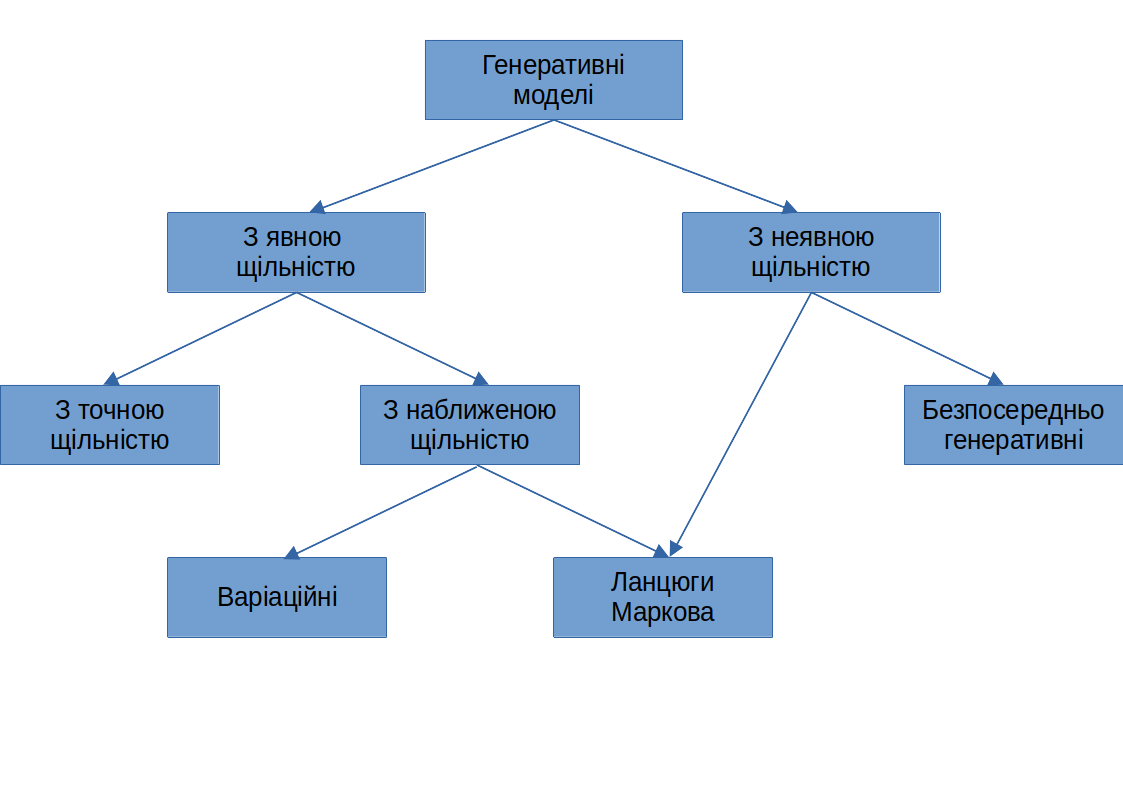
\includegraphics[width=0.9 \textwidth]{gen_models.png}
    \caption{Таксономія генеративних моделей}
    \label{fig:gen_models}
\end{figure}

Моделі з явною щільністю дозволяють обраховувати значення щільності.
Максимізація правдоподібності для даних моделей є простою,
бо являє собою просту підстановку щільності, що описує модель,
у вираз для правдоподібності. Найскладніше для даної групи
підібрати таку модель, яка зможе описувати усю складність реальних даних
і при цьому дозволить обраховувати щільність розподілу.
Тому виділяють дві стратегії:
\begin{enumerate}
    \item моделі, які гарантують можливість точного обрахунку (tractability);
    \item моделі, які ґрунтуються на обрахунку наближених значень.
\end{enumerate}

Моделі, які гарантують можливість точного обрахунку щільності, такі як
FVBN (fully visible belief networks), нормалізуючи потоки, мають перевагу у тому,
що дозволяють проводити оптимізацію безпосередньо функції
правдоподібності, проте це вимагає від них жорстких обмежень.
До того ж більшість подібних моделей виконують обрахунки послідовно,
тобто для генерації необхідно виконати декілька послідовних кроків, які
не можуть бути розпаралелині, що значно збільшує час необхідний для
генерації.

Для уникнення проблем, пов'язаних з жорсткими обмеженнями на
модель, які необхідні для точно обрахунку щільності, використовуються
моделі, які дозволяють отримувати наближені значення щільності.
Вони у свою чергу поділяються на дві групи: з детерміністичною
апроксимацією, здебільшого це автоенкодери, та зі стохастичною,
як наприклад ланцюги Маркова, машини Больцмана.

Звичайно, що і у даних підходів є суттєві недоліки.
Варіаційні автоенкодери використовують у своїй роботі
нижню границю (ELBO), яка при виборі "слабкого" апостеріорного
або ж апріорного може значно відрізнятися від справжньої
правдоподібності, що призведе до того, що розподіл генератора
та реальний розподіл будуть значно відрізнятись. На практиці
варіаційні моделі все ж здатні гарно апроксимувати правдоподібність,
проте якість згенерованих зображень є низькою. Якщо ж казати про
недоліки методів побудованих на основі ланцюгів Маркова, то
слід зазначити їх низьку швидкодію, що обумовлена як необхідністю
виконувати операції покроково, так і тим, що збіжність
дужу повільна та не має жодного методу, який би міг вказати
чи вже наявна збіжність чи потребується продовжити оптимізацію.

Концептуально іншим підходом є застосування моделей, які
не оперують щільністю або її наближеннями як такими, а
навчаються лише ґрунтуючись на тих прикладах, які надає
генератор. Тобто використовують не сам розподіл як такий, а
певні спостереження з нього. Деякі з цих моделей знову ж таки
використовують ланцюги Маркова для генерування прикладів,
здебільшого це генеративні стохастичні мережі. Але вони мають
притаманні усім ланцюгам Маркова недоліки, які були описані вище.
І на сам кінець існують моделі, які здатні безпосередньо
генерувати зображення за один крок. Найбільш відомими й поширеними з них
є генеративно-змагальні мережі, які ми розглянемо більш детально.

\section{Генеративно-змагальні мережі}

Ідея оригінальної GAN  \cite{goodfellow2014generative}
полягає у тому, що ми маємо дві сутності:
генератор --- диференційовну функцію $G: Q \times \Theta_G \rightarrow X$, яка
на основі елементу з множини $Q$ (так званого латентного простору)
та параметрів $\theta_g \in \Theta_G$
генерує елемент з множин $X$; та дискримінатор
--- диференційовну функцію $D: X \times \Theta_D \rightarrow \{0, 1\}$, яка
намагається на визначити чи є елемент штучно згенерованим, чи
належить розподілу навчальних даних. Для пошуку функції
генератора та дискримінатора застосовується міні-максний функціонал якості:
\begin{equation} \label{eq:gan_criterion}
    \min\limits_{G}\max\limits_{D} \left[
        \E_{x \sim \pi} \ln D(x) +
        \E_{q \sim p_{Q}} \ln (1 - D(G(q))) \right],
\end{equation}

Тобто відбувається змагання між генератором, який прагне генерувати найбільш
схожі на реальні зображення, щоб ввести в оману дискримінатор,
який навпаки прагне якомога краще відрізняти штучно згенеровані та
реальні приклади.

Але для того, щоб знайти відповідні оптимальні значення
параметрів дискримінатора та генератора необхідний алгоритм навчання,
який з кожним кроком буде все ближче і ближче наближати розподіл
генератора до реального, аж поки дискримінатор не втратить будь-яку можливість
відрізняти реальні та штучно згенеровані зображення. Дану ідею
зображено на рис. \ref{fig:gan}.

\begin{figure}[h]
    \centering
    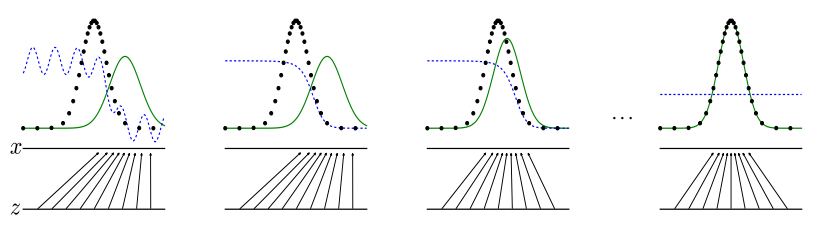
\includegraphics[width=0.75 \textwidth]{gan_distribution.png}
    \caption{Ілюстрація ідеї GAN \cite{goodfellow2014generative}.
        Зеленим позначено розподіл генератора,
        синім --- дискримінатора,
        чорними точками --- реальних даних}
    \label{fig:gan}
\end{figure}

Як це притаманно
штучним нейронним мережам, алгоритм оптимізації ґрунтується на
обрахунку і використанні градієнтів цільової функції помилки
від параметрів. Але, через те, що наша модель не є класичною
нейромережею, необхідний окремий підхід до навчання GAN.

\begin{algorithm}[Алгоритм навчання GAN]

    Параметри: $k$ - кількість ітерацій навчання дискримінатора за 1 епоху,
    $N$ - кількість епох навчання, $m$ - розмірність батчу.

    Вхідні дані: навчальна вибірка $X$ з розподілом $\pi$.

    \begin{enumerate}
        \item Доки кількість епох навчання не досягла $N$
              \begin{enumerate}
                  \item Повторювати $k$ разів
                        \begin{enumerate}[leftmargin=3.25cm]
                            \item Згенерувати $\{z_1, \dots, z_m\}$
                            \item Обрати $\{x_1, \dots, x_m\} \sim \pi(x)$
                            \item Оновити параметри дискримінатора використовуючи градієнт
                                  \begin{equation*}
                                      \nabla_{\theta_D} \left( \frac{1}{m}\sum\limits_{i=1}^m \left[
                                              \ln D(x_i) + \ln (1 - D(G(z_i))) \right] \right)
                                  \end{equation*}
                        \end{enumerate}
                  \item Згенерувати нові $\{z'_1, \dots, z'_m\}$\;
                  \item Оновити параметри генератора використовуючи градієнт
                        \begin{equation*}
                            \nabla_{\theta_G} \left( \frac{1}{m}\sum\limits_{i=1}^m
                            \ln (1 - D(G(z'_i))) \right)
                        \end{equation*}
              \end{enumerate}
    \end{enumerate}
\end{algorithm}

У якості оптимізатора, який використовує вже обраховані градієнти
можна застосовувати довільний алгоритм, у більшості випадків це або
звичайний градієнтний спуск,
або більш досконалі методи, як наприклад
Adam \cite{kingma2014adam}.

Окремим питанням, яке заслуговує на увагу, є питання про те,
а чи дійсно у результаті розв'язку цієї задачі ми отримаємо
генератор, розподіл якого дорівнює розподілу реальних даних.
Для того, щоб переконатися у цьому доведемо дві важливі теореми.

\begin{theorem}[Гудфелоу \cite{goodfellow2014generative}]
    Для фіксованого генератора $G$ з розподілом $p_G(x)$
    оптимальним дискримінатором $D^*(x)$ є:
    \begin{equation*}
        D^{*}(x) = \frac{\pi(x)}{\pi(x) + p_G(x)}.
    \end{equation*}
\end{theorem}
\begin{proof}
    Запишемо цільову функцію:
    \begin{equation*}
        \min\limits_{G}\max\limits_{D} \left[
            \E_{x \sim \pi} \ln D(x) +
            \E_{q \sim p_{Q}} \ln (1 - D(G(q))) \right]
    \end{equation*}
    Генератор, за припущенням є фіксованим, тож ми можемо перейти
    від математичного сподівання по латентному просторі до математичного сподівання
    розподілу генератора $p_G(x)$.
    \begin{equation*}
        \min\limits_{G}\max\limits_{D} \left[
            \E_{x \sim \pi} \ln D(x) +
            \E_{x \sim G(x)} \ln (1 - D(x)) \right]
    \end{equation*}
    Наступним кроком розпишемо математичні сподівання та
    властивостями визначених інтегралів:
    \begin{equation*}
        \min\limits_{G} \int\limits_X \max\limits_{D}
        \left( \pi(x) \ln D(x) +
        p_G(x) \ln (1 - D(x)) \right) dx
    \end{equation*}
    Розглянемо умову екстремум для виразу під
    знаком максимуму і отримаємо:
    \begin{gather*}
        \frac{\partial}{\partial D(x)}
        \left( \pi(x) \ln D(x) +
        p_G(x) \ln (1 - D(x)) \right) = \\
        = \frac{\pi(x)}{D(x)} - \frac{p_G(x)}{1 - D(x)} = 0
    \end{gather*}
    І виразивши $D(x)$ остаточно отримаємо:
    \begin{equation*}
        D^{*}(x) = \frac{\pi(x)}{\pi(x) + p_G(x)}
    \end{equation*}
\end{proof}

\begin{theorem}[Гудфелоу \cite{goodfellow2014generative}]
    Глобальний мінімум критерію \eqref{eq:gan_criterion} досягається
    тобі і тільки тоді, коли розподіли генератора $p_G$ та реальних даних
    однакові. При цьому значення критерію дорівнює $-\ln 4$.
\end{theorem}
\begin{proof}
    Підставимо оптимальний дискримінатор у критерій~\eqref{eq:gan_criterion}.
    \begin{equation*}
        \min\limits_{G} \left[
            \E_{x \sim \pi} \ln \frac{\pi(x)}{\pi(x) + p_G(x)} +
            \E_{q \sim p_G} \ln \frac{\pi_G(x)}{\pi(x) + p_G(x)}
            \right]
    \end{equation*}
    Тепер помножимо і поділимо кожен дріб на 2 та використаємо властивість
    логарифмів та математичного сподівання від константи.
    \begin{equation*}
        \min\limits_{G} \left[
            \E_{x \sim \pi} \ln \frac{2 \pi(x)}{\pi(x) + p_G(x)} +
            \E_{q \sim p_G} \ln \frac{2 \pi_G(x)}{\pi(x) + p_G(x)}
            \right] - \ln 4
    \end{equation*}
    Вираз у дужках є нічим іншим як дивергенцією Йонсена-Шеннона \eqref{eq:jsd}.
    Вона приймає мінімальне значення $0$ тоді і тільки тоді, коли
    розподіли дорівнюють один одному. І, відповідно, значення критерію
    у випадку рівності $0$ мінімуму буде дорівнювати $-\ln 4$.
\end{proof}

Проте наявний алгоритм навчання майже завжди не використовується
на практиці, що пов'язано з тим, що градієнти параметрів генератора
згасають \cite{arjovsky2017towards, goodfellow2014generative}.
Це є наслідком самої будови функції помилки, тому її заміняють
на наступний аналог:

\begin{equation} \label{eq:gan_generator_loss}
    - \ln D(G(z))
\end{equation}

Притаманні процесу навчання генеративно-змагальних мереж і інші проблеми,
як наприклад нестабільність навчання, яка полягає у тому, що
у деяких випадках алгоритм не може знайти оптимальні
дискримінатор та генератор. Деякі причини цього детально
описані у роботі \cite{arjovsky2017towards}, серед них нестабільність
градієнтів функції помилки у вигляді \eqref{eq:gan_generator_loss}.
Іншою можливою причиною може бути те, що як зображено на рис. \ref{fig:gan},
з кожною ітерацією генератор покращується, що робить зворотній
зв'язок від дискримінатора все менш правильним, і на сам кінець зовсім випадковим.
Тобто генератор починає вчитися на небажаному зворотному зв'язку від дискримінатора.

Одним зі шляхів подолання даних проблем є додавання шуму до
входу дискримінатора, застосування спектральних нормалізацій \cite{miyato2018spectral} або
ж регуляризацій \cite{roth2017stabilizing}.

Іншою істотною проблемою є так званий mode collapse.
Вона полягає у тому, що вихідні зображення дуже мало
відрізняються один від одного та модель не в змозі генерувати
різноманітні приклади. Це відбувається через те, що генератор
завжди намагається ввести в оману дискримінатор, і для цього
генерує зображення, які з найбільшою ймовірністю будуть розпізнанні
дискримінатором як справжні. Але якщо виявилось так, що
дискримінатор потрапив у локальний максимум, з якого не може вибратись,
то генератор надмірно пристосовується саме до цього дискримінатора, через
що і генерує невелике розмаїття зображень.

Зміна дискримінатора та критерію оптимізації спроможні подолати
дану проблему. Одним з таких підходів є Wasserstein GAN \cite{arjovsky2017wasserstein}.
Який змінює дискримінатор, який приймає обмежені значення на критика,
виходи якого можуть бути довільні. До того ж сама функція помилки
була змінена на таку, що відображає відстань між розподілами.
Серед усього іншого, даний підхід спроможний допомогти і
у випадку нестабільного навчання.

Попри усі згадані недоліки, якість зображень та швидкодія генерації
штучних прикладів для генеративно-змагальних мереж є
високою, що і робить GAN визнаним спільнотою лідером у задачах
генерації штучних зображень.

Підсумовуючи, генеративно-змагальні мережі мають наступні
переваги над іншими моделями:
\begin{enumerate}
    \item Можливість паралельної генерації,
          що забезпечує швидкість роботи навченої моделі.
    \item На генератора накладається мало обмежень, що дає можливість
          вибору широко класу архітектур.
          Це є перевагою порівняно з машинами Больцмана,
          які допускають лише певні класи  ймовірнісних розподілів,
          а також щодо потоків, що нормалізують, які вимагають, щоб генератор
          мав зворотнє відображення, а розмірність латентного простіру
          дорівнювала розмірності даних.
    \item Не використовуються ланцюги Маркова з усіма їх
          недоліками, як у машинах Больцмана та генеративних стохастичних мережах.
    \item Генеративна мережа, оптимізація якої була збіжною, точно наближає
          розподіл реальних даних, а не використовує нижні чи верхні
          оцінки, як це у випадку з автоенкодерами.
    \item Якість зображень, які генеруються за допомогою GAN,
          здебільшого вища за інші моделі.
\end{enumerate}

Саме ці моменти і обумовлюють вибір саме генеративно-змагальних
мереж для генерації штучних супутникових знімків, і, як наслідок,
аугментації навчальних вибірок.

\section{GAN у задачах image-to-image translation}

Для того, щоб мати вплив на згенеровані класичними
генеративно-змагальними мережами зображення, ми маємо
досліджувати структуру латентного простору, і навіть якщо нам
це, використовуючи певні методи, вдасться, у нас все ще не буде
повного контролю за кожним пікселем зображення, бо
розмірність латентного простору майже завжди менша за
розмірність зображення. Таким чином точно контролювати розподіл класів у
згенерованих зображеннях не є можливим.

Наша ж задача полягає саме у тому, щоб генерувати штучні супутникові
знімки і при цьому мати знання про клас кожного зі згенерованих
пікселів. Саме тому нам потрібно звернути увагу на ті методи, які дозволять
контролювати кожний з вихідних пікселів.

Однією з задач, яка влаштовує наші вимоги є задача image-to-image translation,
яка полягає у тому, що ми повинні перетворити зображення з одного домену у інший, при цьому кількість
каналів вхідного та вихідного зображення не повинна бути однаковою.
Таким чином подавши маски, на яких будуть зазначені класи кожного з пікселів,
ми зможемо генерувати штучні супутникові знімки, з потрібним нам
відношенням класів.

Наївні підходи до розв'язку даної задачі, які полягають у навчанні
звичайної згорткової нейронної мережі з мінімізацією евклідової відстані,
призведуть до того, що значення пікселів кожного з класів будуть
усереднені. І, відповідно, ми отримаємо згенеровані зображення
дуже низької якості. Тож слід звернути увагу на GAN, які дозволять
задати кінцеву ціль у вигляді <<зробити згенеровані
зображення такими, що складно відрізнити від справжніх>>.

Існує цілий клас генеративно-змагальних мереж, які дозволяють вирішувати дану
задачу. Це так звані умовні (conditional) GAN. Однією з провідних
архітектур, саме у задачі image-to-image translation, є Pix2Pix~\cite{pix2pix}.

Першим істотної відмінністю архітектури Pix2Pix від
класичних GAN є функція помилки, а саме: для вхідного зображення
$x$ та бажаного вихідного зображення $y$ вона виглядає
наступним чином:

\begin{equation} \label{eq:pix2pix_loss}
    L(G, D) = \E_{x, y} \log D(x,y) +
    \E_{x} \log (1 - D(x, G(x))) +
    \lambda \E_{y, x} ||y - G(x)||_1
\end{equation}

Тобто функція помилки являє собою поєднання класичної помилки
для генеративно-змагальних мереж, з тією зміною, що дискримінатор приймає
два аргументи, і $L_1$ помилки. Перша частина як і у всіх інших
GAN відповідає за те, щоб згенеровані зображення виглядали подібними
до реальних, а друга частина, намагається досягти
попіксельної однаковості між справжніми та штучними знімками.
$L_1$ помилка була обрана авторами \cite{pix2pix}, бо їх досліди
показали, що використання $L_2$ помилки призводить до більшого
рівня розмитості на вихідних зображеннях.

Наступною відмінністю архітектури Pix2Pix є використання так званого
PatchGAN у якості дискримінатора. Він аналізує справжність не усього
зображення, а лише окремих його частин, і потім усереднює отримані результати.
Це дозволяє ефективно моделювати вихідне зображення як
випадкове поле Маркова, при умові, що припускається
незалежність між пікселями, які потрапили у різні частини.
Це можна розуміти \cite{pix2pix} як текстурну помилку або помилку стилю.

При чому слід звернути увагу на те, що дискримінатор приймає
вхідне та вихідне зображення, тобто має змогу
порівняти а чи відповідає згенероване зображення тому
входу, який був поданий на генератор.

Генератор повинен генерувати вихідне зображення такого ж
розміру який мало вхідне, тож цілком закономірно очікувати,
що архітектура генератора повинна бути більш-менш симетричною.
Однією з таких, добре відомих архітектур, є вже розглянута
нами архітектура UNet. Вона добре зарекомендувала себе у
задачах семантичної сегментації, які дещо схожі на задачу image-to-image translation.
До того ж використання особливості UNet дозволяють враховувати як
високорівневі, так і низькорівневі ознаки. Саме ґрунтуючись на цих
принципах, автори \cite{pix2pix} і запропонували використати
варіацію архітектури UNet у якості генератора.

Таким чином повністю архітектуру Pix2Pix можливо подати за допомогою наступної
діаграми (рис. \ref{fig:pix2pix}).

\begin{figure}[!ht]
    \centering
    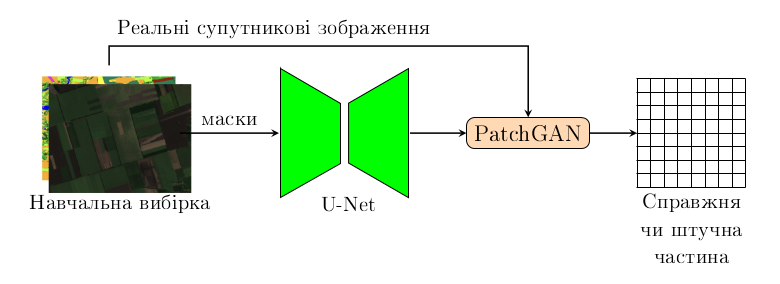
\includegraphics[scale=0.5]{pix2pix.png}
    \caption{Архітектура Pix2Pix у застосуванні до супутникових знімків}
    \label{fig:pix2pix}
\end{figure}

Проте результати роботи запропонованої архітектури інколи
бажають покращення, особливо коли мова йде про генерацію
деталізованих зображень або зображень великої розмірності.
Проте Pix2Pix був і залишається потужною базою, на якій
ґрунтуються більш досконалі методи. Одним з таких є архітектура
Pix2PixHD \cite{pix2pixHD}.

У Pix2PixHD було запропоновано багато вдосконалень класичного
Pix2Pix, серед яких були значні зміни генератора, проте
ці зміни пов'язані з бажанням генерувати саме зображення
більшого розміру. До того ж даний генератор вимагає
більших обчислювальних ресурсів. Ми ж зосередимось на
тих нововведеннях, які мають на меті покращення, у тому числі,
якості зображень.

Першим нововведенням є застосування декількох дискримінаторів.
Кожний з цих дискримінаторів має архітектуру PatchGAN та застосовується
при різних розмірах зображень. Для отримання піраміди зображень
з різними розмірами використовується операція pooling, яка зменшує
у 2 рази. Таким чином різні дискримінатори мають різні рецептивні
поля, що дозволяє їм разом враховувати різні рівні освідомлення
зображення та змінювати генератор так, щоб він генерував
глобально узгоджені результати. Результуюча оцінка ж такого
складеного дискримінатора являє собою суму оцінок кожної
зі складових частин.

Наступні покращення пов'язані з використанням додаткових
функції помилок. Перша з них являє собою так звану помилку
відповідності ознак.

\section{Перспективи застосування GAN для генерації штучних супутникових знімків}

temp

\begin{figure}[!ht]
    \centering
    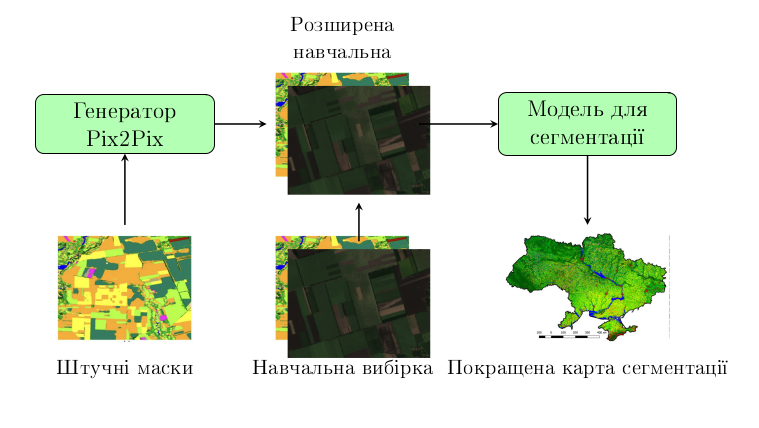
\includegraphics[scale=0.5]{pipline.png}
    \caption{Процес аугментації наборів даних супутникових знімків за допомогою Pix2Pix}
    \label{fig:pipline}
\end{figure}

\begin{algorithm}[Алгоритм генерації масок] \leavevmode \linebreak
    Вхідні дані: навчальна вибірка, бажана кількість пікселів для кожного з класів
    \begin{enumerate}
        \item Визначити які класи не досягли достатньої кількості пікселів та додати їх у чергу
        \item Поки залишились елементи у черзі

              \begin{enumerate}
                  \item Дістати з черги мітку класу $k$
                  \item Для наступного елемента у наборі даних, отримати маску,
                        в якій усі мітки класу, який займає найбільше пікселів замінити
                        на $k$
                  \item Зберегти отриману маску
                  \item Додати кількість міток, які були змінені до
                  сумарної кількості пікселів класу $k$. Якщо для даного
                  класу ще не досягнута бажана кількість пікселів, то додати $k$ у чергу.
              \end{enumerate}
    \end{enumerate}
\end{algorithm}

\chapconclude{\ref{chap:gans}}

У другому розділі ми зосередились на огляді
генеративних моделей та можливостей їх
застосування для аугментації навчальних вибірок
супутникових знімків.

Перш за все було розглянуто постановку задачі
генерування зображень у математичній постановці та
різні класи генеративних моделей. Ґрунтуючись на недоліках і
перевагах кожного з цих класів, було визначено,
що найбільшу перспективу для вирішення задачі генерації
супутникових зображень мають генеративно-змагальні мережі.

Тож було докладно проаналізовано властивості збіжності цих мереж,
наведено алгоритм навчання та описано основні проблеми, які
виникають з GAN та шляхи їх вирішення.

Через те, що задача аугментації вибірок у нашій постановці вимагає
контролю за міткою класу кожного з пікселів згенерованого зображення,
ми звернулись до генеративно-змагальних мереж, які дозволяють
розв'язувати задачу image-to-image translation. Визначними нейромережевими
архітектурами у цій галузі є Pix2Pix та нащадки, тож було
детально проаналізовано їх застосування до
генерації супутникових знімків.

На сам кінець, був запропонований процес аугментації навчальних вибірок супутникових
знімків, який полягає у тому, що ми, за описаним алгоритмом, спершу
генеруємо маски, які будуть коригувати незбалансованість класів,
а після цього, ґрунтуючись на даних масках, генерувати штучні
супутникові знімки за допомогою
архітектури Pix2Pix та її варіацій.
%!TEX root = ../thesis.tex
\chapter{Аналіз застосування GAN для аугментації навчальних вибірок}
\label{chap:practice}

У даному розділі ми застосуємо розглянуті нами у попередніх
частинах моделі та методи на практиці, а саме навчимо варіацію
моделі архітектури UNet з різними функціями помилки. Обрахуємо
метрики і визначимо чи дійсно проблема незбалансованості
класів істотно впливає на якість семантичної сегментації супутникових
знімків. І на сам кінець за допомогою генеративно-змагальних
мереж згенеруємо штучні приклади, які додамо до реальних даних
та будемо проводити навчання вже на ції аугментованій вибірці.
І визначимо чи дійсно подібний спосіб дозволяє
покращити якість семантичної сегментації.

Вихідний код, який був створено для усіх наведених у даному
розділі експериментів доступний на GitHub
\footnote{\href{https://github.com/ShkalikovOleh/SatelliteGAN}
    {https://github.com/ShkalikovOleh/SatelliteGAN}}.

\section{Попередня обробка навчальних даних}

Для перевірки того, чи дійсно запропонований підхід
дозволить збільшити якість семантичної сегментації супутникових знімків
проведемо експерименти з класифікації на 19 класів
композиту Sentinel-2A \cite{drusch2012sentinel}
для Київської області взятих з 1 липня по 1 серпня 2021 року.
Класи представляють собою здебільшого сільськогосподарські
культури, тому розв'язання задачі сегментації саме на таких
даних має широкий прикладний потенціал.

Ми використовували саме композит супутникових знімків, бо
територія Київської області надто велика, щоб вона могла
повністю розміститися на одному супутниковому знімку Sentinel-2A.
Саме тому був взятий часовий ряд червоного, зеленого, синього та
ближнього інфрачервоного каналів за липень 2021~р., який потім був об'єднаний.
У тих частинах, що перетиналися були, були обрані медіанні значення
пікселів, також знімки були очищені від детектованих хмар та тіней від них.

Після чого ці дана колекція знімків була об'єднана у один
великий композит для Київської області та до цього композиту
була додана окремим каналом маска з мітками класів, яка була
отримана у результаті досліджень науковцями інституту
космічних досліджень Національної академії наук України.

Сучасні нейромережеві архітектури не дозволяють нам працювати
з зображення дуже великого розміру, тому ми вимушені
розрізати отриманий композит на квадратні частини розміром $256 \times 256$
пікселів. Такий вибір обґрунтований тим, що саме такий розмір
зображення генерувався авторами класичного Pix2Pix  \cite{pix2pix}.

Попри те, що ми брали дані за місяць, все одно залишились
території, які не були покриті супутником за спостережуваний період.
До того ж, контури Київської області не є ідеальною геометричною фігурою,
тож на деяких знімках, на яких показані кордони області відсутні значення
пікселів або масок, які відповідають іншим областям.
Через ці два фактори у деяких отриманих зображеннях
присутні пікселі, у яких відсутнє значення.
Такі приклади були відфільтровані та не
використовувалися при навчанні нейронних мереж.

На сам кінець, через те, що використовувалися знімки з
попередньою обробкою та корекцією класу TOA, то
область значень кожного з каналів була не класичною
$[0, 1]$, а мала більше максимальне значення.
У свою чергу більшість нейромережевих архітектур працює зі
значеннями у проміжку $[-1, 1]$.
Тож був застосований аналог min-max нормалізації, а саме
кожне значення пікселю кожного каналу було поділено на
максимальне значення для даного каналу даного зображення,
а після цього класична стандартизація з математичним
сподівання і стандартним відхиленням рівними $0.5$.

\section{Результати сегментації без використання GAN}

Для розв'язання задачі семантичної сегментації
даної вибірки супутникових знімків було використано
архітектуру UNet. Для того, щоб ми мали змогу перевірити
якість моделі використовуючи метрики, і при цьому
отримали достовірні значення, тобто уникнули явища
перенавчання, вибірку було поділено навпіл на навчальну і тестову.

У якості енкодера у використаній варіації UNet було обрано
ResNet-34, що є компромісом між обчислювальною потужністю,
необхідною для навчання подібних моделей та
складністю мережі.

Дана вибірка є незбалансованою, що можна побачити на
статистиках по сумарній кількості пікселів
для кожного класів на рисунку \ref{fig:pixels_per_class}
(мітки класів відповідають назвам, які можна знайти
у таблиці \ref{tab:segm_result_real_per_classes}).
Тож для подолання проблем, які пов'язані з цим, ми спробували
застосувати різні функції помилок, а саме зважені та
не зважені Cross-Entropy
та Focal Loss. У якості вагових коефіцієнтів для кожного
класу були обрані нормовані зворотні відношення сумарної кількості пікселів класу
до кількості усіх пікселів у тренувальній вибірці.

У якості оптимізатора було обрано добре відомий,
один з найбільш застосовуваних та ефективних,
алгоритм Adam \cite{kingma2014adam} зі швидкістю навчання
$2 \cdot 10^{-4}$. Розмір батчу дорівнював $64$.

\begin{table}[!ht]
    \centering
    \caption{Глобальні метрики точності сегментації
        для реальної вибірки}
    \begin{tabular}{|c|C|C|C|C|}
        \hline
        \multirow{2}{*}{Метрика} & \multicolumn{2}{c|}{CE Loss} & \multicolumn{2}{c|}{Focal Loss}                                   \\
        \cline{2-5}              & w/o W                        & W                               & w/o W          & W              \\
        \hline $\acc$            & 0.76                         & 0.738                           & \textbf{0.762} & 0.755          \\
        \hline $\varkappa$       & 0.72                         & 0.697                           & \textbf{0.722} & 0.716          \\
        \hline $\iou$            & 0.356                        & 0.352                           & 0.363          & \textbf{0.368} \\
        \hline
    \end{tabular}
    \label{tab:segm_result_real_global}
\end{table}

У результаті $500$-та епох навчання було отримані значення
метрик, таких як точність ($\acc$), міра Жаккара ($\iou$) та
каппа Коена ($\varkappa$), для різних варіацій функції помилки.
Вони наведені у таблиці \ref{tab:segm_result_real_global}
(w/o W означає не зважену помилку, W -- зважену).

Що стосується якості сегментації за кожним з класів, то
слід звернутися до таких метрик як Producer Accuracy $\pracc$
та User Accuracy $\usacc$, наведених у таблиці \ref{tab:segm_result_real_per_classes}.

\begin{table}[!ht]
    \centering
    \caption{Метрики точності сегментації за класами
        для реальної вибірки}
    \begin{tabular}{|K|C|C|C|C|C|C|C|C|}
        \hline
        \multirow{3}{*}{Назва класу}   & \multicolumn{4}{c|}{PA}         & \multicolumn{4}{c|}{UA}                                                                                                               \\
        \cline{2-9}
                                       & \multicolumn{2}{c|}{CE Loss}    & \multicolumn{2}{c|}{Focal Loss} &
        \multicolumn{2}{c|}{CE Loss}   & \multicolumn{2}{c|}{Focal Loss}                                                                                                                                         \\
        \cline{2-9}
                                       & w/o W                           & W                               & w/o W          & W              & w/o W          & W              & w/o W          & W              \\
        \hline Штучні об'єкти          & 0.64                            & \textbf{0.66}                   & 0.649          & 0.652          & 0.664          & 0.59           & \textbf{0.68}  & 0.668          \\
        \hline Зернові культури        & 0.822                           & 0.772                           & \textbf{0.825} & 0.791          & 0.718          & 0.712          & 0.721          & 0.734          \\
        \hline Ріпак                   & 0.285                           & 0.285                           & 0.272          & \textbf{0.297} & \textbf{0.533} & 0.404          & 0.533          & 0.458          \\
        \hline Гречка                  & 0.012                           & 0.038                           & 0.032          & \textbf{0.047} & 0.151          & 0.059          & \textbf{0.165} & 0.1            \\
        \hline Кукурудза               & 0.882                           & 0.825                           & \textbf{0.887} & 0.861          & 0.837          & \textbf{0.853} & 0.834          & 0.85           \\
        \hline Буряк                   & 0.27                            & 0.356                           & 0.324          & \textbf{0.367} & 0.472          & 0.417          & \textbf{0.537} & 0.435          \\
        \hline Соняшник                & \textbf{0.887}                  & 0.848                           & 0.881          & 0.866          & 0.83           & 0.83           & 0.839          & \textbf{0.844} \\
        \hline Соя                     & 0.581                           & \textbf{0.64}                   & 0.595          & 0.608          & 0.715          & 0.584          & \textbf{0.716} & 0.662          \\
        \hline Інші культури           & 0.09                            & \textbf{0.207}                  & 0.09           & 0.201          & 0.222          & 0.162          & \textbf{0.233} & 0.192          \\
        \hline Ліс                     & 0.915                           & 0.827                           & \textbf{0.918} & 0.897          & 0.894          & \textbf{0.931} & 0.897          & 0.913          \\
        \hline Необроблювані землі     & 0.726                           & 0.592                           & \textbf{0.741} & 0.686          & 0.683          & \textbf{0.723} & 0.692          & 0.716          \\
        \hline Відкритий ґрунт         & 0.464                           & 0.694                           & 0.494          & \textbf{0.696} & \textbf{0.573} & 0.392          & 0.57           & 0.438          \\
        \hline Вода                    & \textbf{0.967}                  & 0.964                           & 0.962          & 0.959          & 0.939          & 0.927          & \textbf{0.94}  & \textbf{0.94}  \\
        \hline Болото                  & 0.315                           & \textbf{0.5}                    & 0.308          & 0.434          & 0.461          & 0.287          & \textbf{0.476} & 0.369          \\
        \hline Ячмінь                  & 0.205                           & \textbf{0.292}                  & 0.206          & 0.28           & 0.309          & 0.265          & \textbf{0.317} & 0.3            \\
        \hline Горох                   & 0.01                            & \textbf{0.018}                  & 0.014          & 0.016          & 0.101          & 0.03           & \textbf{0.135} & 0.075          \\
        \hline Трави                   & 0.011                           & \textbf{0.051}                  & 0.016          & 0.038          & 0.083          & 0.05           & 0.1            & \textbf{0.111} \\
        \hline Сади, парки, лісополоси & 0.51                            & 0.496                           & \textbf{0.522} & 0.495          & 0.491          & 0.433          & \textbf{0.498} & 0.486          \\
        \hline Виноградники            & 0.039                           & 0.344                           & 0.01           & \textbf{0.345} & 0.169          & 0.09           & \textbf{0.197} & 0.144          \\
        \hline
    \end{tabular}
    \label{tab:segm_result_real_per_classes}
\end{table}

Як можна побачити, за усіма метриками, які є глобальними
перевагу має нейромережа архітектури UNet, яка
при навчанні використовувала не зважену функцію
помилки FocalLoss, а саме вона переважає у Accuracy та
каппі Коена, у той же час відставання за метрикою $\iou$
від лідера не значне.

Що стосується результатів метрик за
кожним окремим класом, то тут бачимо той факт, що як і
очікувалось ті класі, які є міноритарними, тобто кількість їх
пікселів мала відносно інших класів, мають значно нижчі показника,
аніж мажоритарні. Але і для цих метрик мережа, що
навчалась з не зваженим Focal Loss видає переважно кращі
результати, особливо, якщо звернути увагу
на User Accuracy, де така варіацію UNet переважає
для 11 класів, більшість з яких саме міноритарні.
Значення метрики Producer Accuracy теж є достатньо
високими: за 5 класами підхід з використання цієї функції
помилки є найкращими (у той час як лідер переважає у
7 класах), а для інших теж показує гарні результати.

\section{Результати сегментації з використанням аугментованого набору даних}

Як ми переконались, незбалансованість класів дуже
істотно впливає на якість семантичної сегментації супутникових
знімків. Тож спробуємо доповнити нашу вибірку, таким чином збалансувавши її.
Для цього використаємо розроблений нами процес аугментації
за допомогою генеративно-змагальних мереж.

\subsection{Генерація доповнених вибірок}

Перш за все були навчені GAN архітектури Pix2Pix та її варіацію
(будемо позначати її Pix2Pix + HD),
що використовує ті покращення, що
описані у розділі \ref{chap:gans}, а саме:
декілька дискримінаторів та функції помилки узгодженості
ознак~\eqref{eq:fm_loss} та узгодженості внутрішніх представлень
навченої мережі класифікації~\eqref{eq:perceptual_loss}.

Навчання відбувалося протягом 500 епох з використання
оптимізатора Adam \cite{kingma2014adam} зі швидкістю навчання
$2 \cdot 10^{-4}$. У якості параметрів експоненційного
середнього ($\beta_1, \beta_2$) використовувались
значення $0.5, 0.999$ відповідно. Розмір батчу був невеликий і
дорівнював $8$, бо великі значення можуть приводити до
зниження якості згенерованих зображень.

Приклади справжніх зображень (лише червоний, зелений та синій канал)
та тих, які генерують навченні
генеративно-змагальні мережі наведені на рисунках
\ref{fig:real_examples} -- \ref{fig:gen_pix2pix_hd_examples}.

\begin{figure}[ht]
    \centering
    \begin{subfigure}[b]{0.3\textwidth}
        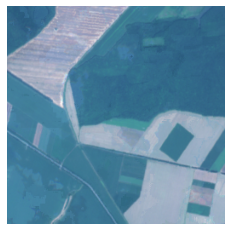
\includegraphics[scale=0.5]{real_0.png}
    \end{subfigure}
    \begin{subfigure}[b]{0.3\textwidth}
        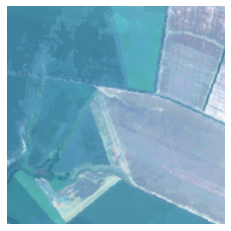
\includegraphics[scale=0.5]{real_1.png}
    \end{subfigure}
    \begin{subfigure}[b]{0.3\textwidth}
        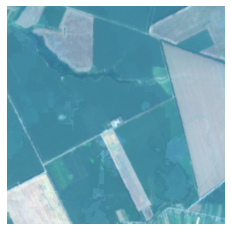
\includegraphics[scale=0.5]{real_2.png}
    \end{subfigure}
    \caption{Приклади справжніх супутникових знімків}
    \label{fig:real_examples}
\end{figure}

\begin{figure}[ht]
    \centering
    \begin{subfigure}[b]{0.3\textwidth}
        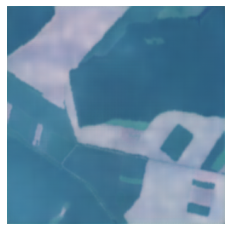
\includegraphics[scale=0.5]{gen_pix2pix_0.png}
    \end{subfigure}
    \begin{subfigure}[b]{0.3\textwidth}
        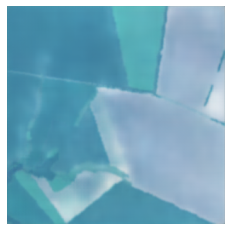
\includegraphics[scale=0.5]{gen_pix2pix_1.png}
    \end{subfigure}
    \begin{subfigure}[b]{0.3\textwidth}
        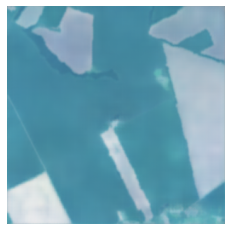
\includegraphics[scale=0.5]{gen_pix2pix_2.png}
    \end{subfigure}
    \caption{Приклади згенерованих Pix2Pix зображень}
    \label{fig:gen_pix2pix_examples}
\end{figure}

\begin{figure}[ht]
    \centering
    \begin{subfigure}[b]{0.3\textwidth}
        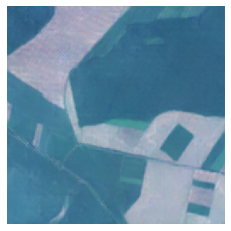
\includegraphics[scale=0.5]{gen_pix2pix_hd_0.png}
    \end{subfigure}
    \begin{subfigure}[b]{0.3\textwidth}
        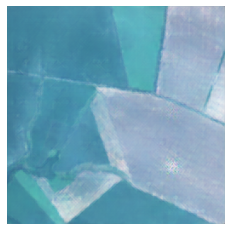
\includegraphics[scale=0.5]{gen_pix2pix_hd_1.png}
    \end{subfigure}
    \begin{subfigure}[b]{0.3\textwidth}
        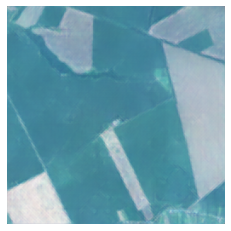
\includegraphics[scale=0.5]{gen_pix2pix_hd_2.png}
    \end{subfigure}
    \caption{Приклади згенерованих Pix2Pix + HD зображень}
    \label{fig:gen_pix2pix_hd_examples}
\end{figure}

Як ми бачимо, на згенерованих прикладах присутня
деяка розмитість та інші незначні артефакти, проти
вони виглядають наближеними до справжніх. Причому візуально
знімки згенеровані модифікацією Pix2Pix виглядають краще.
До того ж,
як ми вже зазначали, кінцевою нашою метою є саме покращення
якості сегментації, а не генерація ідеальних зображень.


Наступним етапом було застосування алгоритму \ref{alg:mask_gen} генерації
штучних масок. Як можна побачити на рисунку \ref{fig:real_examples}
у досліджуваному наборі даних дуже сильний дисбаланс у кількості
пікселів для кожного з класів, тому якщо ми будемо намагатися
зробити повністю рівномірний розподіл, то нам потрібно буде
згенерувати дуже багато штучних зображень, що
може тільки зменшити метрики якості семантичної сегментації.
Тож було обрано наступний підхід: за цільові значення кількості пікселів
обрано $70\%$ від кількості пікселів класу <<Зернові культури>>.
У якості параметру $l$ алгоритму було обрано $2$. При чому
у прикладних застосуваннях нас цікавить підвищення якості класифікації не усіх
класів, а лише окремих, як наприклад нас не цікавить розпізнавання
штучних об'єктів, у тому числі будинків та автомобілів,
якщо ми вирішуємо задачі, які пов'язані з сільськогосподарськими
культурами. Тож ми використали властивість розробленого алгоритму,
яка полягає у тому, що він дозволяє обирати
класи, які будуть доповнюватись, та доповнили наступні класи:
ріпак, гречка, буряк, соя, інші культури, виноградники, трави,
горох, ячмінь.

Усього було згенеровано $1252$ нових приклади кожної з навчених
генеративно-змагальних мереж, і усі вони були додані до
вихідної тренувальної вибірки, таким чином ми отримали аугментовану вибірку.
Статистика по кількості пікселів у доповненій вибірці наведена на
рисунку \ref{fig:pixels_per_class_aug}. Як можна побачити,
класи, які нас особливо цікавлять, стали набагато більш збалансовані.

\begin{figure}[ht!]
    \centering
    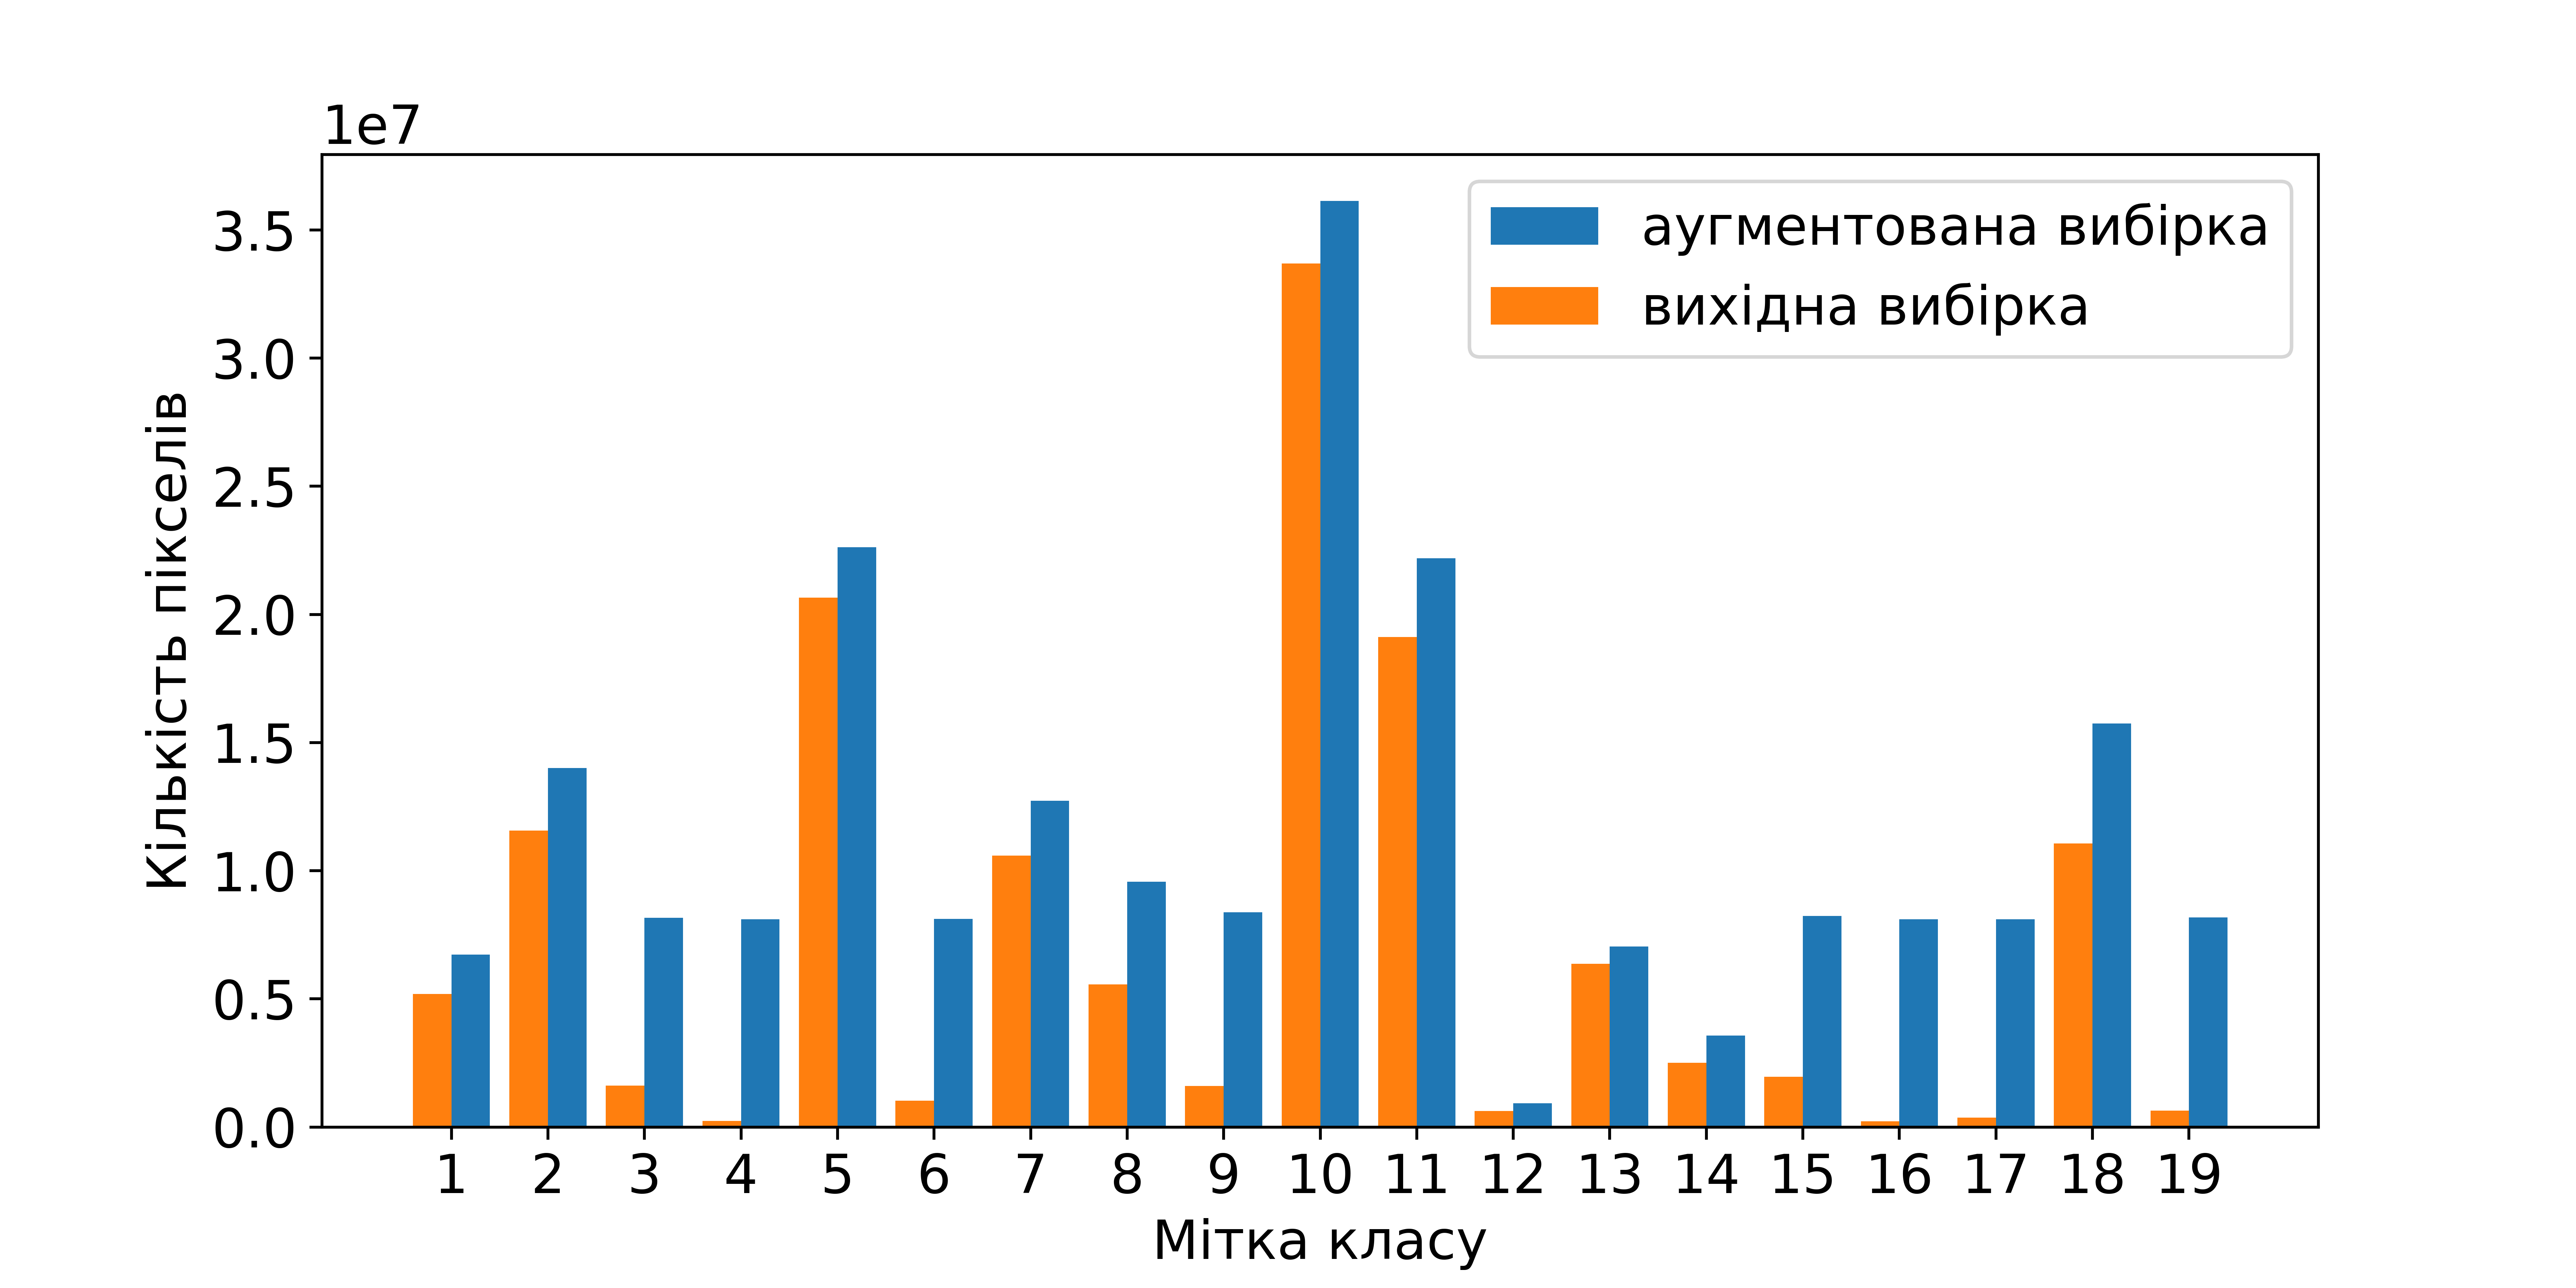
\includegraphics[scale=0.65]{dist_aug_real.png}
    \caption{Порівняння кількості пікселів для різних класів
        у досліджуваному та аугментованому наборах даних}
    \label{fig:pixels_per_class_aug}
\end{figure}

\subsection{Аналіз якості семантичної сегментації при застосуванні
    доповнених вибірок}

Маючи аугментовану вибірку ми маємо змогу перейти до перевірки
нашої гіпотези про те, що генеративно-змагальні мережі
здатні допомогти підвищити якість семантичної сегментації. Для цього,
щоб порівнювати з результатами на вихідній навчальній вибірці,
ми теж навчаємо мережу архітектури UNet з енкодером ResNet-34.
Усі параметри навчання були обрані таки ми же, окрім кількості
епох, яка була зменшена до $300$ через те, що ми працюємо з
більшою вибіркою.

Результати у вигляді глобальних метрик наведені у таблиці \ref{tab:segm_result_aug_global}.
Найкращі показники має

\newcolumntype{S}{>{\centering\arraybackslash}m{1.3cm}}
\newcolumntype{M}{>{\centering\arraybackslash}p{2.2cm}}

\begin{table}[!ht]
    \centering
    \caption{Порівняння глобальних метрик
        точності сегментації
        для доповненої вибірки та вихідної вибірок}
    \begin{tabular}{|c|S|C|C|}
        \hline
        \multirow{2}{*}{Метрика} & \multirow{2}{1.3cm}{Вихідна вибірка} & \multicolumn{2}{M|}{Аугментована вибірка}                \\
        \cline{3-4}              &                                      & Pix2Pix                                   & Pix2Pix + HD \\
        \hline $\acc$            & 0.762                                & 79                                        & 4            \\
        \hline $\varkappa$       & 0.722                                & 0.715                                     & 4            \\
        \hline $\iou$            & 0.363                                & 79                                        & 4            \\
        \hline
    \end{tabular}
    \label{tab:segm_result_aug_global}
\end{table}

Якщо ж казати, про метрики точності по класам, то вони наведені у таблиці
\ref{tab:segm_result_augm_per_classes}.

\begin{table}[!ht]
    \centering
    \caption{Порівняння метрик
        точності сегментації за кожним класом
        для доповненої вибірки та вихідної вибірок}
    \begin{tabular}{|K|S|C|C|S|C|C|}
        \hline
        \multirow{3}{*}{Назва класу}         & \multicolumn{3}{c|}{PA}                   & \multicolumn{3}{c|}{UA}                                                              \\
        \cline{2-7}
                                             & \multirow{2}{1.3cm}{Вихідна вибірка}      & \multicolumn{2}{M|}{Аугментована вибірка} &
        \multirow{2}{1.3cm}{Вихідна вибірка} & \multicolumn{2}{M|}{Аугментована вибірка}                                                                                        \\
        \cline{3-4} \cline{6-7}
                                             &                                           & Pix2Pix                                   & Pix2Pix + HD &  & Pix2Pix & Pix2Pix + HD \\
        \hline Штучні об'єкти                & 0.649                                     &                                           &              &  &         &              \\
        \hline Зернові культури              & 0.825                                     &                                           &              &  &         &              \\
        \hline Ріпак                         & 0.272                                     &                                           &              &  &         &              \\
        \hline Гречка                        & 0.032                                     &                                           &              &  &         &              \\
        \hline Кукурудза                     & 0.887                                     &                                           &              &  &         &              \\
        \hline Буряк                         & 0.324                                     &                                           &              &  &         &              \\
        \hline Соняшник                      & 0.881                                     &                                           &              &  &         &              \\
        \hline Соя                           & 0.595                                     &                                           &              &  &         &              \\
        \hline Інші культури                 & 0.09                                      &                                           &              &  &         &              \\
        \hline Ліс                           & 0.918                                     &                                           &              &  &         &              \\
        \hline Необроблювані землі           & 0.741                                     &                                           &              &  &         &              \\
        \hline Відкритий ґрунт               & 0.494                                     &                                           &              &  &         &              \\
        \hline Вода                          & 0.962                                     &                                           &              &  &         &              \\
        \hline Болото                        & 0.308                                     &                                           &              &  &         &              \\
        \hline Ячмінь                        & 0.206                                     &                                           &              &  &         &              \\
        \hline Горох                         & 0.014                                     &                                           &              &  &         &              \\
        \hline Трави                         & 0.016                                     &                                           &              &  &         &              \\
        \hline Сади, парки, лісополоси       & 0.522                                     &                                           &              &  &         &              \\
        \hline Виноградники                  & 0.01                                      &                                           &              &  &         &              \\
        \hline
    \end{tabular}
    \label{tab:segm_result_augm_per_classes}
\end{table}

Отримані результати свідчать про те, що

\chapconclude{\ref{chap:practice}}
Перемога


% Створюємо висновки
\conclusions
%!TEX root = ../thesis.tex
% створюємо Висновки до всієї роботи
У результаті проведеної роботи була досліджена проблема
семантичної сегментації супутникових знімків, яка має важливу
роль у прикладних застосуваннях. Проте були виявлені та описані
проблеми, які виникають під час розв'язку цієї задачі сучасними
нейромережевими методами, а саме: складність створення великих
вибірок та сильна незбалансованість класів. Причому, на відміну від
інших сфер, отримати навчальні приклади, які могли б змінити розподіл
класів у багатьох випадках для супутникових даних не є можливим.

Для подолання цих проблем було розглянуто можливість аугментації
навчальної вибірки штучно згенерованими навчальними прикладами.
Для цього була дослідженні моделі, які дозволяють вирішити цю задачу,
а саме генеративно-змагальні мережі. При цьому, для вирішення проблеми
незбалансованості класів стандартні GAN не кращий вибір, бо
ми не можемо контролювати розподіл класів на згенерованих зображеннях.
Тому були опрацьовані моделі image-to-image translation, зокрема Pix2Pix,
які дозволяють генерувати супутникові знімки на основі масок.
У свою чергу модифікація вже існуючих масок, тобто зміна одних
класів на інші дозволяє скоригувати незбалансованість класів.

Таким чином було розроблено процес аугментації наборів даних супутникових
знімків, ефективність якого була перевірена
експериментальним чином (табл. \ref{tab:segm_result_augm_per_classes}, \ref{tab:segm_result_aug_global}).
Для генерації були використані різні модифікації
архітектури Pix2Pix, у тому числі та, яка
використовує дискримінатор та функції помилки з
архітектури Pix2PixHD, яка показала кращі результати, як з точки
зору метрик семантичної сегментації так і за якістю згенерованих
зображень.

Також було проведено дослідження різних функції помилки, які
застосовні при навчанні модифікації архітектури UNet, яка безпосередньо
і відповідає за семантичну сегментацію. Серед усіх досліджуваних підходів
найкращим виявився той, що використовував не зважену функцію похибки
Focal Loss. Його ж ми і застосовували при навчанні моделей
вже на доповнених вибірках.

У результаті ми отримали підтвердження того, що запропонований
підхід дозволяє значно підвищити якість семантичної сегментації
міноритарних класів, при цьому якість класифікації мажоритарних класів, хоч
у деяких випадках і стала нижчою, проте незначно.

Очевидні і подальші напрямки досліджень у даній сфері. По-перше, це
дослідження методів генерації, які б дозволили б врахувати той факт,
що супутникові знімки однієї території у різні пори року значно відрізняються.
По-друге, створення більш досконалих методів генерації масок.
І врешті решт, покращення існуючих генеративно-змагальних мереж
для генерації ще більш реалістичних штучних супутникових знімків.


% Додаємо бібліографію

% \bibliographystyle{ugost2008}
\bibliographystyle{utf8gost780u}
\renewcommand\bibname{Перелік посилань}
\pagebreak
\addcontentsline{toc}{chapter}{Перелік посилань}
\bibliography{thesis}

\end{document}